
Let {\color{black}$D \subsetneq \RPat_{\Sigma\cup X}$} with $\sharp D = 2$ or $3$, and let $p,q$ be regular patterns in {\color{black}$\RPat_{\Sigma\cup X}$}.
In the following subsections (Subsecs.~\ref{subsec:d2}--\ref{subsec:d3c}), we provide the conditions on $D$ under which the implication holds: if $p \{ x := r \} \preceq q$ for all $r \in D$, then $p \{ x := xy \} \preceq q$.
It is obvious if the variable symbol $x$ does not occur in $p$.
Therefore, in the following lemmas and propositions, let $p=p_{1}xp_{2}$, where {\color{black}$p_{i}\in \RPat_{\Sigma\cup X}$} ($i=1,2$) and $x$ is a variable symbol.

{\color{black}
Lemma 14 (ii) of \cite{Sato1} stated that, when $\sharp \Sigma \geq 3$, for regular patterns $p,q$, if $p\{x:=r\}\preceq q$ for any $r\in D$, then $p\{x:=xy\} \preceq q$, where 
$D = \{ a_{1}b_{1}, a_{2}b_{2}, a_{3}b_{3}\}$ $(a_{i} \ne a_{j} \mbox{ and } b_{i} \ne b_{j} \mbox{ for each } i,j~(i\ne j, 1\le i,j\le 3))$.
Unfortunately, there exist the following counterexamples of Lemma 14 (ii) of \cite{Sato1}.
\begin{ex}\label{CounterExample_Lemma14}
Assume that $a_1=b_2$ and $a_3=b_1$.
{\color{black} In the following two examples, we have $p\{x:=r\}\preceq q$ for $r\in D$}.
  
\begin{itemize}
\item[(1)] 
Let $p=ca_1xa_3c$ and $q=ya_1a_3z$ {\color{black} where $c$ is a symbol in $\Sigma$}.
It is clear that $p\{x:=xy\} \not\preceq q$.
However, we have $p\{x:=a_1b_1\}\preceq q$, $p\{x:=a_2b_2\}\preceq q$ and $p\{x:=a_3b_3\}\preceq q$, 
since
$p\{x:=a_1b_1\}=ca_1a_1b_1a_3c=q\{y:=ca_1,z:=a_3c\}$,
$p\{x:=a_2b_2\}=ca_1a_2b_2a_3c=q\{y:=ca_1a_2,z:=c\}$ and 
$p\{x:=a_3b_3\}=ca_1a_3b_3a_3c=q\{y:=c,z:=b_3a_3c\}$.

\item[(2)] 
Let $p=cb_2a_1b_1b_2xa_1b_1b_2a_3c$ and $q=yb_2a_1b_1b_2a_3z$  {\color{black} where $c$ is a symbol in $\Sigma$}.
It is clear that $p\{x:=xy\} \not\preceq q$.
However, we have that $p\{x:=a_1b_1\}\preceq q$, $p\{x:=a_2b_2\} \preceq q$ and $p\{x:=a_3b_3\} \preceq q$ hold, 
since  
$p\{x:=a_1b_1\}=cb_2a_1b_1b_2a_1b_1a_1b_1b_2a_3c=q\{y:=cb_2a_1b_1,z:=b_2a_3c\}$,
$p\{x:=a_2b_2\}=cb_2a_1b_1b_2a_2b_2a_1b_1b_2a_3c=q\{y:=cb_2a_1b_1b_2a_2,z:=c\}$,
and  $p\{x:=a_3b_3\}=cb_2a_1b_1b_2a_3b_3a_1b_1b_2a_3c=q\{y:=c,z:=b_3a_1b_1b_2a_3c\}$.
\end{itemize}
\end{ex}
}

{\color{black}For regular patterns $p,q\in\RPat$ with $p\not\preceq q$, we} consider the correspondence from $r\in D$ to some string in $q$ when $p \{ x := r \} \preceq q$.
The symbols in $D$ correspond to either a variable or a constant symbol in $q$.
If $D$ has a constant string $ab$ of length $2$ for $a,b\in\Sigma$, there are three possible strings in $q$ that correspond to $ab$ in $p\{x:=ab\}$ as follows: For $y_{1} \in X$,
  \begin{center}
    \begin{tabular}{cccccc}
      \textrm{(a)} & $ab$, & \textrm{(b)} & $ay_{1}$, & \textrm{(c)} & $y_{1}b$.
    \end{tabular}
  \end{center}

\noindent
If there exists $ay_{1}$ in $q$ that corresponds to $ab$, i.e., there exist $q_{1}$ and $q_{2}\in \RPat$ such that
  \begin{enumerate}
  \item[(1)] $p_{1}abp_{2} \preceq q_{1}ay_{1}q_{2}$, 
  \item[(2)] $p_{1} \preceq q_{1}$, and
  \item[(3)] either $p_{2} \preceq q_{2}$ or $p_{2} \preceq y_{1}^{\prime}q_{2}$ for $y_{1}^{\prime}\in X$.
  \end{enumerate}
Let $D^{\prime} = (D \setminus \{ab\}) \cup \{ay\}$.
It is straightforward to see that $p\{x:=ay\} = p_{1}ayp_{2} \preceq q_{1}ay_{1}q_{2}$.
Thus, $p \{ x := r \} \preceq q$ for all $r \in D^{\prime}$.
Let $D^{\prime\prime} = (D \setminus \{ab\}) \cup \{yb\}$.
By a similar discussion, if there exists $y_{1}b$ in $q$ that corresponds to $ab$, $p \{ x := r \} \preceq q$ for all $r \in D^{\prime\prime}$.
Therefore, in this paper, we make the following definition on $D$:

\smallskip

\begin{dfn}
Let $p,q \in \RPat$ {\color{black} with $p\not\preceq q$}.
Let $D \subsetneq \RPat$ such that for all $r\in D$, $|r| = 2$ and $p \{ x := r \} \preceq q$.
Then, if for any $ab\in D$ ($a,b\in\Sigma$), {\color{black} $ay,yb\not\in D$}, $p \{ x := ay \} \not\preceq q$ and $p \{ x := yb \} \not\preceq q$ for any $y \in X$ that does not occur in $q$,
{\color{black}the regular pattern $q$ is said to \textit{minimally support $D$ for $p$}, in the sense that any generalization of the strings in $D$ would invalidate the conditions $p\{x := r\} \preceq q$ for all $r\in D$}.

\end{dfn}

\noindent{\color{black} In Subsecs.~\ref{subsec:d3a}--\ref{subsec:d3c}, we consider a subset $D \subsetneq \RPat_{\Sigma\cup X}$ such that a regular pattern $q \in \RPat_{\Sigma\cup X}$ minimally support $D$ for a regular pattern $p$.} 


\subsection{$D=\{ ay, by \}$ and $D=\{ ya, yb \}$}\label{subsec:d2}

{\color{red}
\begin{prop}[Unique Factorization w.r.t. a Fresh Variable]\label{prop:fresh_var_factorization}
Let $\alpha_1, \alpha_2, \beta_1, \beta_2 \in (\Sigma \cup X)^*$ and let $y \in X$ be a variable symbol. 
If $y$ does not occur in $\alpha_1, \alpha_2, \beta_1, \beta_2$ (i.e., $y \notin \mathrm{var}(\alpha_1\alpha_2\beta_1\beta_2)$) and
$\alpha_1 y \alpha_2 = \beta_1 y \beta_2$, 
then $\alpha_1 = \beta_1$ and $\alpha_2 = \beta_2$.
\end{prop}

\begin{proof}
Consider the free monoid $(\Sigma \cup X)^*$. 
Since $y$ does not appear in $\alpha_1$ or $\beta_1$, the symbol $y$ appears exactly once in $\alpha_1 y \alpha_2$ at index $|\alpha_1| + 1$, and exactly once in $\beta_1 y \beta_2$ at index $|\beta_1| + 1$. 
Since the two strings are identical, the unique occurrence of the symbol $y$ must be at the identical index. 
Thus, $|\alpha_1| = |\beta_1|$.
Since $\alpha_1$ and $\beta_1$ are prefixes of the same string having the same length, it follows that $\alpha_1 = \beta_1$. 
Cancelling $\alpha_1 y$ (or $\beta_1 y$) from the left yields $\alpha_2 = \beta_2$.
\end{proof}

\begin{lem}[Boundary Absorption Lemma]\label{lem:boundary-absorption}
Let $p = p_1 x p_2 \in \mathcal{RP}$ with $x \in X$, and let $q \in \mathcal{RP}$. 
Let $a, b \in \Sigma$ with $a \neq b$, and let $y \in X$ be a fresh variable occurring in neither $p$ nor $q$ ($y \notin \mathrm{var}(p) \cup \mathrm{var}(q)$).
Assume that there exist substitutions $\theta_a$ and $\theta_b$ such that
\begin{equation}\label{eq:hyp_images}
q\theta_a = p_1 a y p_2 \quad \text{and} \quad q\theta_b = p_1 b y p_2.
\end{equation}
Suppose there exists a variable $z \in \mathrm{var}(q)$ and strings $u, v \in (\Sigma \cup X)^*$ satisfying
\begin{equation}\label{eq:z_images}
z\theta_a = u a y v \quad \text{and} \quad z\theta_b = u b y v,
\end{equation}
and for every variable $t \in \mathrm{var}(q) \setminus \{z\}$, $t\theta_a = t\theta_b$.
Then,
$
p\{x := x y\} \preceq q.
$
\end{lem}

\begin{proof}
Since $q$ is regular, the variable $z$ occurs exactly once in $q$. Hence we can write
\[
q = q_L z q_R
\]
for some patterns $q_L, q_R \in (\Sigma \cup X)^*$ with $z \notin \mathrm{var}(q_L) \cup \mathrm{var}(q_R)$. From $q\theta_a = p_1 a y p_2$ and $z\theta_a = u a y v$, we obtain
\[
(q_L\theta_a)(u a y v)(q_R\theta_a) = p_1 a y p_2,
\]
which is rewritten as
\[
(q_L\theta_a u a) y (v q_R\theta_a) = (p_1 a) y p_2.
\]
Since $y$ is fresh and does not occur in $q_L\theta_a, q_R\theta_a, u, v, p_1$, or $p_2$, Proposition~4 implies
\begin{align}
q_L\theta_a u a &= p_1 a, \\
v q_R\theta_a &= p_2.
\end{align}
Cancelling the final symbol $a$ from the first equality yields
\[
q_L\theta_a u = p_1.
\]
Define a substitution $\sigma$ by
\begin{align*}
z\sigma &= u x y v, \\
t\sigma &= t\theta_a \quad \text{for every } t \in \mathrm{var}(q) \setminus \{z\}.
\end{align*}
This is a valid substitution because $u x y v$ is non-empty ($|u x y v| \ge |x y| = 2 \ge 1$) and $|\theta_a(t)| \ge 1$ for all $t \neq z$. Then, since $z$ does not occur in $q_L$ and $q_R$, we have $q_L\sigma = q_L\theta_a$ and $q_R\sigma = q_R\theta_a$. Thus,
\begin{align*}
q\sigma &= (q_L\sigma)(z\sigma)(q_R\sigma) \\
        &= (q_L\theta_a)(u x y v)(q_R\theta_a) \\
        &= (q_L\theta_a u) x y (v q_R\theta_a) \\
        &= p_1 x y p_2 \\
        &= p\{x := x y\}.
\end{align*}
Therefore, $p\{x := x y\} \preceq q$, which shows that the lemma holds.
\end{proof}

\begin{lem}[Boundary Extension Lemma] \label{lem:boundary-extension} 
  Let $p=p_1xp_2$ and let $q\in RP_{\Sigma\cup X}$. Let $a,b\in\Sigma$ with $a\neq b$ and let $y$ be a fresh variable. 
  Assume $p\{x:=ay\}\preceq q, p\{x:=by\}\preceq q. $
  Suppose that the occurrence of $a$ which corresponds to the first symbol of the factor replacing $x$ is not immediately followed by a variable occurrence in $q$. 
  Then $p\{x:=xy\}\preceq q. $
\end{lem} 
\begin{proof} 
Since $y \notin \mathrm{var}(q)$ and $q\theta_a = p_1 a y p_2$, the fresh variable $y$ must be generated by the substitution $\theta_a$ acting on some variable of $q$.
Because $y$ occurs exactly once in $p_1 a y p_2$ and $q$ is a regular pattern, there exists a unique variable $z \in \mathrm{var}(q)$ such that $y$ occurs in $z\theta_a$.

Thus, $q$ can be uniquely decomposed as
\[
q = q_L z q_R,
\]
where $q_L, q_R \in (\Sigma \cup X)^*$ and $z \notin \mathrm{var}(q_L) \cup \mathrm{var}(q_R)$. Moreover, $z\theta_a$ is uniquely decomposed as
\[
z\theta_a = u_a y v,
\]
where $u_a, v \in (\Sigma \cup X)^*$ and $y \notin \mathrm{var}(q_L\theta_a) \cup \mathrm{var}(q_R\theta_a) \cup \mathrm{var}(u_a) \cup \mathrm{var}(v)$.

\paragraph{Step 1: Prefix and Suffix Factorization under $\theta_a$.}
Expanding $q\theta_a$ yields:
\[
q\theta_a = (q_L\theta_a)(z\theta_a)(q_R\theta_a) = (q_L\theta_a u_a) y (v q_R\theta_a).
\]
Equating this with $q\theta_a = (p_1 a) y p_2$ and applying Proposition~4, we obtain:
\begin{align}
q_L\theta_a u_a &= p_1 a, \label{eq:lem5_left}\\
v q_R\theta_a &= p_2. \label{eq:lem5_right}
\end{align}

\paragraph{Step 2: Proving $u_a$ Ends with $a$.}
We analyze equation (\ref{eq:lem5_left}). The right-hand side ends with the constant symbol $a \in \Sigma$.
Suppose, for contradiction, that $u_a = \varepsilon$. Then (\ref{eq:lem5_left}) implies $q_L\theta_a = p_1 a$.
In this case, the final symbol $a$ of $q_L\theta_a$ corresponds to the end of $q_L$. By the hypothesis of the lemma, $q$ does not contain $az$ as a factor (i.e., the occurrence of $a$ is not immediately followed by $z$ in $q$). Therefore, $u_a \neq \varepsilon$.

Since $u_a \neq \varepsilon$, the trailing constant symbol $a$ of $p_1 a$ in (\ref{eq:lem5_left}) must originate from the suffix of $u_a$. Consequently, there exists a string $u \in (\Sigma \cup X)^*$ such that
\begin{equation}\label{eq:lem5_u_decomp}
u_a = ua \quad \text{and} \quad q_L\theta_a u = p_1.
\end{equation}
Hence, we obtain
\begin{equation}\label{eq:lem5_z_theta_a}
z\theta_a = u a y v.
\end{equation}

\paragraph{Step 3: Construction of Modified Substitution $\theta'_b$.}
We define a substitution $\theta'_b \colon (\Sigma \cup X)^* \to (\Sigma \cup X)^*$ on variables as follows:
\[
t\theta'_b = 
\begin{cases}
u b y v & \text{if } t = z, \\
t\theta_a & \text{if } t \in \mathrm{var}(q) \setminus \{z\}.
\end{cases}
\]
Since $|u b y v| \ge |b y| = 2 \ge 1$ and $|\theta_a(t)| \ge 1$ for all $t \neq z$, $\theta'_b$ is a well-defined substitution.

We verify that $q\theta'_b = p_1 b y p_2$. Because $z \notin \mathrm{var}(q_L) \cup \mathrm{var}(q_R)$, the substitution $\theta'_b$ acts identically to $\theta_a$ on $q_L$ and $q_R$, which means $q_L\theta'_b = q_L\theta_a$ and $q_R\theta'_b = q_R\theta_a$. Thus:
\begin{align*}
q\theta'_b &= (q_L\theta'_b)(z\theta'_b)(q_R\theta'_b) \\
           &= (q_L\theta_a)(u b y v)(q_R\theta_a) \\
           &= (q_L\theta_a u) b y (v q_R\theta_a).
\end{align*}
Substituting (\ref{eq:lem5_u_decomp}) and (\ref{eq:lem5_right}) into this expansion:
\[
q\theta'_b = p_1 b y p_2 = p\{x := by\}.
\]

\paragraph{Step 4: Application of Lemma~\ref{lem:boundary-absorption}.}
The substitutions $\theta_a$ and $\theta'_b$ satisfy all the requirements of Lemma~\ref{lem:boundary-absorption} (Boundary Absorption Lemma):
\begin{enumerate}
    \item $q\theta_a = p_1 a y p_2$ and $q\theta'_b = p_1 b y p_2$,
    \item $z\theta_a = u a y v$ and $z\theta'_b = u b y v$,
    \item $t\theta'_b = t\theta_a$ for every variable $t \in \mathrm{var}(q) \setminus \{z\}$.
\end{enumerate}
Therefore, by Lemma~\ref{lem:boundary-absorption}, we conclude:
\[
p\{x := xy\} \preceq q.
\]\end{proof}

\begin{prop}[Factorization of Instance over Concatenation]\label{prop:factorization}
Let $p, q_A, q_B \in \mathcal{RP}_{\Sigma \cup X}$. If $p \preceq q_A q_B$ (i.e., there exists a substitution $\theta$ such that $q_A\theta q_B\theta = p$), then there exist patterns $p_A, p_B \in (\Sigma \cup X)^*$ such that:
\begin{enumerate}
    \item $p = p_A p_B$,
    \item $p_A \preceq q_A$ with $q_A\theta = p_A$,
    \item $p_B \preceq q_B$ with $q_B\theta = p_B$.
\end{enumerate}
\end{prop}
\begin{proof}
Since $\theta$ is a monoid homomorphism on $(\Sigma \cup X)^*$, we have $(q_A q_B)\theta = (q_A\theta)(q_B\theta) = p$. Setting $p_A = q_A\theta$ and $p_B = q_B\theta$, the concatenation equality $p = p_A p_B$ holds immediately, and by definition $p_A \preceq q_A$ and $p_B \preceq q_B$ under the same substitution $\theta$.
\end{proof}

\begin{lem}\label{lem:lemma6_fixed}
Let $p = p_1 x p_2 \in \mathcal{RP}_{\Sigma \cup X}$ and let $q \in \mathcal{RP}_{\Sigma \cup X}$. Let $a, b \in \Sigma$ with $a \neq b$, and let $y \in X$ be a fresh variable ($y \notin \mathrm{var}(p) \cup \mathrm{var}(q)$).
Assume that
\[
p\{x := ay\} \preceq q, \quad p\{x := by\} \preceq q, \quad \text{and} \quad p\{x := xy\} \not\preceq q.
\]
Then there exist regular patterns $q_1, q_2 \in \mathcal{RP}_{\Sigma \cup X}$, distinct variables $y_1, y_2 \in \mathrm{var}(q)$, and a string $w \in \Sigma^*$ such that either
\begin{equation}\label{eq:form1}
q = q_1 a y_1 w b y_2 q_2 \quad \text{or} \quad q = q_1 b y_1 w a y_2 q_2.
\end{equation}
\end{lem}

\begin{proof}
Let $\theta_a$ and $\theta_b$ be substitutions such that
\[
q\theta_a = p_1 a y p_2 \quad \text{and} \quad q\theta_b = p_1 b y p_2.
\]
Since $y \notin \mathrm{var}(q)$ and $y$ occurs exactly once in each of $p_1 a y p_2$ and $p_1 b y p_2$, and since $q$ is a regular pattern, the fresh variable $y$ must be generated by a unique variable in $q$ under $\theta_a$ and $\theta_b$, respectively.
Let $z_a, z_b \in \mathrm{var}(q)$ be the unique variables such that $y \in \mathrm{var}(z_a\theta_a)$ and $y \in \mathrm{var}(z_b\theta_b)$.

\paragraph{Step 1: Distinctness of $z_a$ and $z_b$ via Explicit Verification of Lemma~5.}
We prove $z_a \neq z_b$ by contradiction. Suppose, to the contrary, that $z_a = z_b = z$.
Since $q \in \mathcal{RP}_{\Sigma \cup X}$ is regular, $z$ occurs exactly once in $q$. Hence, $q$ is uniquely decomposed as
\[
q = q_L z q_R,
\]
where $q_L, q_R \in (\Sigma \cup X)^*$ and $z \notin \mathrm{var}(q_L) \cup \mathrm{var}(q_R)$.
Furthermore, since $y \in \mathrm{var}(z\theta_a)$ and $y$ occurs uniquely in $q\theta_a$, $z\theta_a$ factorizes uniquely as
\[
z\theta_a = u_a y v_a
\]
for some strings $u_a, v_a \in (\Sigma \cup X)^*$ with $y \notin \mathrm{var}(u_a) \cup \mathrm{var}(v_a) \cup \mathrm{var}(q_L\theta_a) \cup \mathrm{var}(q_R\theta_a)$.

Expanding $q\theta_a$:
\[
q\theta_a = (q_L\theta_a)(u_a y v_a)(q_R\theta_a) = (q_L\theta_a u_a) y (v_a q_R\theta_a) = (p_1 a) y p_2.
\]
By Proposition~4 (Unique Factorization with respect to a Fresh Variable), we obtain
\begin{equation}\label{eq:step1_fact_a}
q_L\theta_a u_a = p_1 a \quad \text{and} \quad v_a q_R\theta_a = p_2.
\end{equation}

We now examine whether $u_a = \varepsilon$:
\begin{itemize}
    \item Suppose, for contradiction, that $u_a \neq \varepsilon$. Then the trailing constant symbol $a$ of $p_1 a$ in (\ref{eq:step1_fact_a}) must come from the suffix of $u_a$. Thus, $u_a = ua$ for some string $u \in (\Sigma \cup X)^*$, which yields $z\theta_a = u a y v_a$ and $q_L\theta_a u = p_1$.
    In this case, the occurrence of $a$ immediately preceding $y$ in $q\theta_a$ is generated within the substitution image of $z$, and $q$ does not contain $az$ as an explicit factor preceding $z$.
    
    We now verify that all hypotheses of Lemma~5 (Boundary Extension Lemma) are satisfied:
    \begin{enumerate}
        \item[(i)] $p = p_1 x p_2 \in \mathcal{RP}_{\Sigma \cup X}$ and $q \in \mathcal{RP}_{\Sigma \cup X}$;
        \item[(ii)] $a, b \in \Sigma$ with $a \neq b$, and $y \in X$ is a fresh variable ($y \notin \mathrm{var}(p) \cup \mathrm{var}(q)$);
        \item[(iii)] $p\{x := ay\} \preceq q$ and $p\{x := by\} \preceq q$ both hold by assumption;
        \item[(iv)] $z$ is the unique variable in $q$ whose image under $\theta_a$ contains $y$;
        \item[(v)] The occurrence of $a$ immediately preceding $y$ in $q\theta_a$ is generated within the image $z\theta_a$ (i.e., $q$ does not contain $az$ as a factor).
    \end{enumerate}
    Since all conditions (i)--(v) are strictly verified, Lemma~5 applies directly and concludes $p\{x := xy\} \preceq q$. However, this contradicts the hypothesis $p\{x := xy\} \not\preceq q$.
    Therefore, we must have $u_a = \varepsilon$.
\end{itemize}

Since $u_a = \varepsilon$, equation (\ref{eq:step1_fact_a}) becomes $q_L\theta_a = p_1 a$. Because $a \in \Sigma$ is a constant symbol and substitution images cannot be empty ($|\theta_a(t)| \ge 1$ for all variables $t$), the final symbol $a$ in $q_L\theta_a$ must originate from an explicit constant symbol $a$ at the end of $q_L$ (i.e., $q_L = q_L' a$). Thus, $q = q_L' a z q_R$, meaning that the factor $az$ explicitly appears in $q$.

By symmetric reasoning on $\theta_b$ with $z\theta_b = u_b y v_b$, if $u_b \neq \varepsilon$, Lemma~5 symmetrically yields $p\{x := xy\} \preceq q$, which contradicts $p\{x := xy\} \not\preceq q$. Hence $u_b = \varepsilon$, which implies $q_L\theta_b = p_1 b$, and thus $q_L$ must end with the constant symbol $b$ (i.e., $q = q_L'' b z q_R$).

However, $q$ is a regular pattern, so the single occurrence of the variable $z$ in $q$ can be preceded by at most one symbol in $q_L$. Since $a \neq b$, $q$ cannot contain both $az$ and $bz$ preceding the same variable $z$ simultaneously.
This contradiction completes the proof that
\[
z_a \neq z_b.
\]

\paragraph{Step 2: Occurrence of Factors $a y_1$ and $b y_2$ in $q$.}
Since $z_a \in \mathrm{var}(q)$ is the unique variable generating $y$ under $\theta_a$, we decompose $z_a\theta_a = u_a y v_a$.
As proved in Step~1, if $u_a \neq \varepsilon$, then all conditions of Lemma~5 are fulfilled, which would imply $p\{x := xy\} \preceq q$, contradicting the hypothesis.
Therefore, $u_a = \varepsilon$, which implies $q_L\theta_a = p_1 a$, and hence $q$ contains $a z_a$ as an explicit factor with $z_a\theta_a = y v_a$. We define $y_1 = z_a$. Thus, $q$ contains the factor $a y_1$.

Symmetrically, under $\theta_b$, the variable $z_b$ generating $y$ must satisfy $u_b = \varepsilon$ to avoid $p\{x := xy\} \preceq q$ via Lemma~5. This implies that $q$ contains $b z_b$ as an explicit factor with $z_b\theta_b = y v_b$. We define $y_2 = z_b$. Thus, $q$ contains the factor $b y_2$.

Since $y_1 \neq y_2$ (by Step~1) and $q$ is regular (each variable occurs at most once), one of the factors $a y_1$ or $b y_2$ must appear strictly before the other in $q$.
Without loss of generality, assume that $a y_1$ precedes $b y_2$ in $q$ (the case where $b y_2$ precedes $a y_1$ is symmetric).
Then $q$ is uniquely partitioned as:
\[
q = q_1 a y_1 w b y_2 q_2
\]
for some patterns $q_1, q_2 \in (\Sigma \cup X)^*$ and $w \in (\Sigma \cup X)^*$.

\paragraph{Step 3: Proving $w \in \Sigma^*$.}
We now show that $w$ contains no variable symbols.
Suppose, for contradiction, that $w$ contains at least one variable symbol $z \in \mathrm{var}(w)$.
Then $w$ can be decomposed as $w = w_L z w_R$ with $w_L, w_R \in (\Sigma \cup X)^*$ and $z \notin \mathrm{var}(w_L)$.

Under $\theta_a$, since $y_1\theta_a = y v_1$ (where $v_1 = v_a$), the equality $q\theta_a = (p_1 a) y p_2$ yields
\[
q_1\theta_a = p_1 \quad \text{and} \quad v_1 (w_L z w_R b y_2 q_2)\theta_a = p_2.
\]
Under $\theta_b$, since $y_2\theta_b = y v_2$ (where $v_2 = v_b$), the prefix of $q\theta_b = p_1 b y p_2$ up to the factor $b y_2$ matches $p_1 b$, which yields
\[
(q_1 a y_1 w_L z w_R)\theta_b = p_1.
\]
We explicitly define a substitution $\tau \colon (\Sigma \cup X)^* \to (\Sigma \cup X)^*$ on variables as follows:
\[
t\tau = 
\begin{cases}
t\theta_b & \text{if } t \in \mathrm{var}(q_1 a y_1 w_L), \\
(z\theta_b)(w_R\theta_b) \cdot x y \cdot v_1 (w_L\theta_a)(z\theta_a) & \text{if } t = z, \\
t\theta_a & \text{if } t \in \mathrm{var}(w_R b y_2 q_2).
\end{cases}
\]
Since $q$ is a regular pattern, the variable sets $\mathrm{var}(q_1 a y_1 w_L)$, $\{z\}$, and $\mathrm{var}(w_R b y_2 q_2)$ are pairwise disjoint.
Furthermore, $|z\tau| \ge |xy| = 2 \ge 1$ and $|\theta_a(t)| \ge 1, |\theta_b(t)| \ge 1$ for all variables $t$, so $\tau$ is a well-defined substitution homomorphism.

Evaluating $q\tau$:
\begin{align*}
q\tau &= (q_1 a y_1 w_L)\tau \cdot (z\tau) \cdot (w_R b y_2 q_2)\tau \\
      &= (q_1 a y_1 w_L)\theta_b \cdot \Big( (z\theta_b)(w_R\theta_b) \cdot x y \cdot v_1(w_L\theta_a)(z\theta_a) \Big) \cdot (w_R b y_2 q_2)\theta_a \\
      &= \Big( (q_1 a y_1 w_L)\theta_b (z\theta_b) (w_R\theta_b) \Big) \cdot x y \cdot \Big( v_1 (w_L\theta_a)(z\theta_a) (w_R b y_2 q_2)\theta_a \Big) \\
      &= (q_1 a y_1 w_L z w_R)\theta_b \cdot x y \cdot v_1 (w_L z w_R b y_2 q_2)\theta_a \\
      &= p_1 x y p_2 \\
      &= p\{x := xy\}.
\end{align*}
This implies $p\{x := xy\} \preceq q$, which directly contradicts the assumption $p\{x := xy\} \not\preceq q$.
Therefore, $w$ cannot contain any variable symbols, which establishes $w \in \Sigma^*$ and completes the proof.
\end{proof}
  }

\begin{lem}\label{lem:twovariables}
%Let $\Sigma$ be an alphabet with $\sharp\Sigma \ge 3$.
{\color{black}Let $\Sigma$ be an alphabet with $\sharp\Sigma \ge 2$}.
Let $p,q$ be regular patterns in {\color{black}$\RPat_{\Sigma\cup X}$}.
Let $D$ be the following set of regular patterns in $\RPat_{\Sigma\cup X}$, where $y$ is a variable symbol that does not occur in $p$ and $q$:
\begin{enumerate}
\item[{\rm (i)}] $D=\{ ay, by \}$ ($a \not= b$),
\item[{\rm (ii)}] $D=\{ ya, yb \}$ ($a \not= b$).
\end{enumerate}
Then, if $p \{ x := r \} \preceq q$ for all $r \in D$, then $p \{ x := xy \} \preceq q$.
\end{lem}

\begin{proof}
%
%{\color{black}
%Case \textrm{(ii)} follows from case \textrm{(i)} by symmetry, upon reversing the strings $p$ and $q$.
%}
%Therefore, in the following, we consider only the case of \textrm{(i)}: $D=\{ ay, by \}$ ($a \not= b$).
%{\color{black} We will prove the case $p\not\preceq q$, since the case $p\preceq q$ is trivial.}
%{\color{black} Since $p\not\preceq q$, but $p_{1}ayp_{2}\preceq q$ and $p_{1}byp_{2}\preceq q$ hold, it follows from Theorem~\ref{Sato1:Lemma9} that
%there exist regular patterns $q_{1},q_{2}$ {\color{black}over} $\Sigma\cup X$ such that $q=q_{1}ay_{1}wby_{2}q_{2}$ or $q=q_{1}by_{1}way_{2}q_{2}$ for some variable symbols $y_{1},y_{2}$ with $y_{1} \not= y_{2}$, and a constant string $w\in \Sigma^{*}$ with $|w|\geq 0$.
%}
%
%When $q=q_{1}ay_{1}wby_{2}q_{2}$, the following four conditions hold: For $y_{1}^{\prime}, y_{2}^{\prime}\in X$,
%\begin{align*}
%\textrm{(1)} & ~p_{1} \preceq q_{1}, & \textrm{(1')} & ~p_{2} \preceq wby_{2}q_{2} \mbox{~or~}\\
%& & & p_{2} \preceq y_{1}^{\prime}wby_{2}q_{2},\\
%\textrm{(2)} & ~p_{1} \preceq q_{1}ay_{1}w, & \textrm{(2')} & ~p_{2} \preceq q_{2} \mbox{~or~}
%p_{2} \preceq y_{2}^{\prime}q_{2}.
%\end{align*}
%
%From (2), there exist regular patterns $p_{1}^{\prime},p_{1}^{\prime\prime}$ such that $p_{1}=p_{1}^{\prime}p_{1}^{\prime\prime}$, $p_{1}^{\prime} \preceq q_{1}a$ and $p_{1}^{\prime\prime} \preceq y_{1}w$.
%Therefore, since $p=p_{1}xp_{2}=p_{1}^{\prime}p_{1}^{\prime\prime}xp_{2}$,
%if $p_{2} \preceq wby_{2}q_{2}$ of (1') holds, 
%$p\preceq q_{1}ap_{1}^{\prime\prime}xwby_{2}q_{2}\equiv q \{ y_{1} := p_{1}^{\prime\prime}x \}$.
%{\color{black} Hence, $p\{x:=xy\}\preceq q$.}
%If $p_2\preceq y_{1}^{\prime}wby_{2}q_{2}$ of (1') holds, $p\preceq q_{1}ap_{1}^{\prime\prime}xy_{1}^{\prime}wby_{2}q_{2}=q \{ y_{1} := p_{1}^{\prime\prime}xy_{1}^{\prime} \}$.
%Thus, $p\{x := xy\} \preceq q \{ y_{1} := p_{1}^{\prime\prime}xyy_{1}^{\prime} \}$.
%{\color{black} Hence, $p\{x:=xy\}\preceq q$.}
%Therefore, we conclude that if $p \{ x := r \} \preceq q$ for all $r \in \{ ay, by \}$ with $a \not= b$, then $p \{ x := xy \} \preceq q$.
%
%%%
{\color{red}
%Case (ii) follows from case (i) by symmetry, upon reversing the strings $p$ and $q$. 
%Therefore, in the following, we consider only the case (i): $D = \{ay, by\}$ ($a \ne b$).
%
%If $p \preceq q$ holds, then clearly $p\{x := xy\} \preceq q$. Thus, it suffices to show that $p\{x := r\} \preceq q$ for all $r \in \{ay, by\}$ implies $p \preceq q$.
%
%If at least one of the substrings $ay$ or $by$ is entirely absorbed by a single variable symbol in $q$, then $p = p_1 x p_2 \preceq q$ immediately holds. 
%Otherwise, since $a \ne b$, the substrings $ay$ and $by$ must match distinct constant-variable pairs in $q$. 
%Since $q$ is a regular pattern, there exist regular patterns $q_1, q_2, w$ over $\Sigma \cup X$ and distinct variable symbols $y_1, y_2 \in X$ such that $q = q_1 a y_1 w b y_2 q_2$ or $q = q_1 b y_1 w a y_2 q_2$. Without loss of generality, assume $q = q_1 a y_1 w b y_2 q_2$.
%
%Since $p_1 a y p_2 \preceq q$ and $p_1 b y p_2 \preceq q$, the following conditions must hold for some $y'_1, y'_2 \in X$:
%\begin{align}
%    &(1)\ p_1 \preceq q_1, &&(1')\ p_2 \preceq w b y_2 q_2 \quad\text{or}\quad p_2 \preceq y'_1 w b y_2 q_2, \tag{1}\\
%    &(2)\ p_1 \preceq q_1 a y_1 w, &&(2')\ p_2 \preceq q_2 \quad\text{or}\quad p_2 \preceq y'_2 q_2. \tag{2}
%\end{align}
%From (2), there exist regular patterns $p'_1, p''_1$ such that $p_1 = p'_1 p''_1$ with $p'_1 \preceq q_1 a$ and $p''_1 \preceq y_1 w$. 
%Since $q$ is a regular pattern, the variable sets occurring in $q_1$ and $w b y_2 q_2$ are mutually disjoint, allowing their corresponding substitutions to be applied independently.
%
%If $p_2 \preceq w b y_2 q_2$ in (1') holds, then
%\[
%p = p_1 x p_2 = p'_1 p''_1 x p_2 \preceq q_1 a p''_1 x w b y_2 q_2 = q\{y_1 := p''_1 x\}.
%\]
%Hence, $p \preceq q$.
%
%If $p_2 \preceq y'_1 w b y_2 q_2$ in (1') holds, then
%\[
%p = p_1 x p_2 = p'_1 p''_1 x p_2 \preceq q_1 a p''_1 x y'_1 w b y_2 q_2 = q\{y_1 := p''_1 x y'_1\}.
%\]
%Hence, $p \preceq q$.
%
%In all cases, we obtain $p \preceq q$, which immediately implies $p\{x := xy\} \preceq q$.}
%
Case (ii) follows from Case (i) by symmetry, upon reversing the strings $p$ and $q$. Hence, it suffices to consider only Case (i), namely $D=\{ay,by\}$ with $a\neq b$. Assume, for contradiction, that \[ p\{x:=xy\}\not\preceq q. \] Since \[ p\{x:=ay\}\preceq q \quad\text{and}\quad p\{x:=by\}\preceq q, \] Lemma~\ref{lem:lemma6_fixed} implies that \[ q=q_1ay_1wby_2q_2 \] or \[ q=q_1by_1way_2q_2, \] for some regular patterns $q_1,q_2$, distinct variables $y_1,y_2$, and a string $w\in\Sigma^*$. We consider only the former case, since the latter is symmetric. Then the following conditions hold for some variables $y'_1,y'_2\in X$: \begin{align} p_1 &\preceq q_1, \tag{1}\\ p_2 &\preceq wby_2q_2 \quad\text{or}\quad p_2\preceq y'_1wby_2q_2, \tag{1'}\\ p_1 &\preceq q_1ay_1w, \tag{2}\\ p_2 &\preceq q_2 \quad\text{or}\quad p_2\preceq y'_2q_2. \tag{2'} \end{align} From (2), there exist regular patterns $p'_1$ and $p''_1$ such that \[ p_1=p'_1p''_1, \] \[ p'_1\preceq q_1a, \] and \[ p''_1\preceq y_1w. \] Suppose first that \[ p_2\preceq wby_2q_2. \] Then \[ \begin{aligned} p\{x:=xy\} &= p_1xyp_2 \\ &= p'_1p''_1xyp_2 \\ &\preceq q_1a(p''_1xy)wby_2q_2 \\ &= q\{y_1:=p''_1xy\}. \end{aligned} \] Hence \[ p\{x:=xy\}\preceq q, \] contrary to the assumption. Next suppose that \[ p_2\preceq y'_1wby_2q_2. \] Then \[ \begin{aligned} p\{x:=xy\} &= p_1xyp_2 \\ &= p'_1p''_1xyp_2 \\ &\preceq q_1a(p''_1xyy'_1)wby_2q_2 \\ &= q\{y_1:=p''_1xyy'_1\}. \end{aligned} \] Again, \[ p\{x:=xy\}\preceq q, \] contrary to the assumption. Therefore both possibilities lead to contradictions. Thus \[ p\{x:=xy\}\preceq q. \] Hence the lemma holds.}
\end{proof}



Let $p$ and $q$ be regular patterns in {\color{black}$\RPat_{\Sigma\cup X}$}.
In this paper, the statement like Lemma~\ref{lem:twovariables} is illustrated by a bipartite graph $(\Sigma, \Sigma, E)$ where $E = \{(a, b) \in \Sigma\times\Sigma \mid p\{x:=ab\} \preceq q\}$.
For example, the conditions (i) and (ii) in Lemma~\ref{lem:twovariables} are illustrated in (1) and (2) in Fig.~\ref{fig:lem4bigraph}, respectively.

\begin{figure}[t]
  \begin{center}
    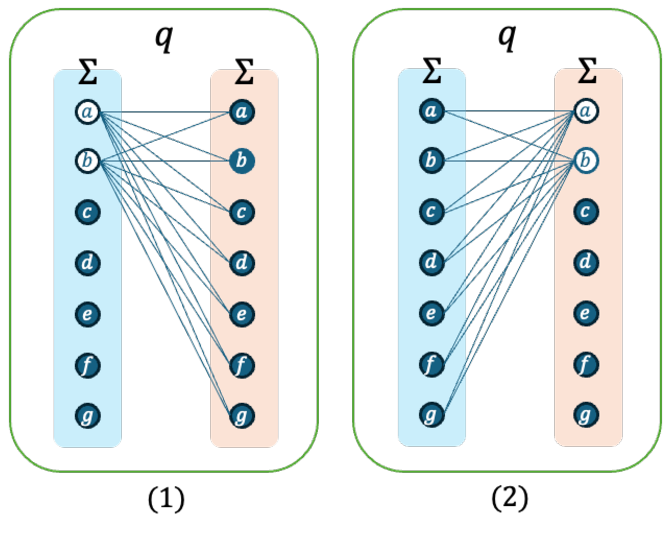
\includegraphics[scale=0.525]{figs/lem4bigraph.pdf}
    \caption{Let $\Sigma=\{a,b,c,d,e,f,g\}$ and $p,q \in {\color{black}\RPat_{\Sigma\cup X}}$. We assume that the symbols in $\Sigma$ are mutually distinct.
    These figures (1) and (2) express two cases $D = \{ ay, by \}$ and $D = \{ ya, yb \}$, respectively.
    In these cases, if $p \{ x := r \} \preceq q$ for all $r \in D$, then $p \{ x := xy \} \preceq q$.}\label{fig:lem4bigraph}
  \end{center}
\end{figure}